
\item O bloco de \SI{5}{\kilogram} é solto do repouso em $A$. Determine a compressão de cada uma das molas após o bloco atingir a plataforma e ser levado instantaneamente ao repouso. Inicialmente, ambas as molas não estão deformadas. Suponha que a plataforma tenha massa desprezível.

\import{answers/}{answer-4}

\vspace{-1.6cm}
\begin{flushright}
    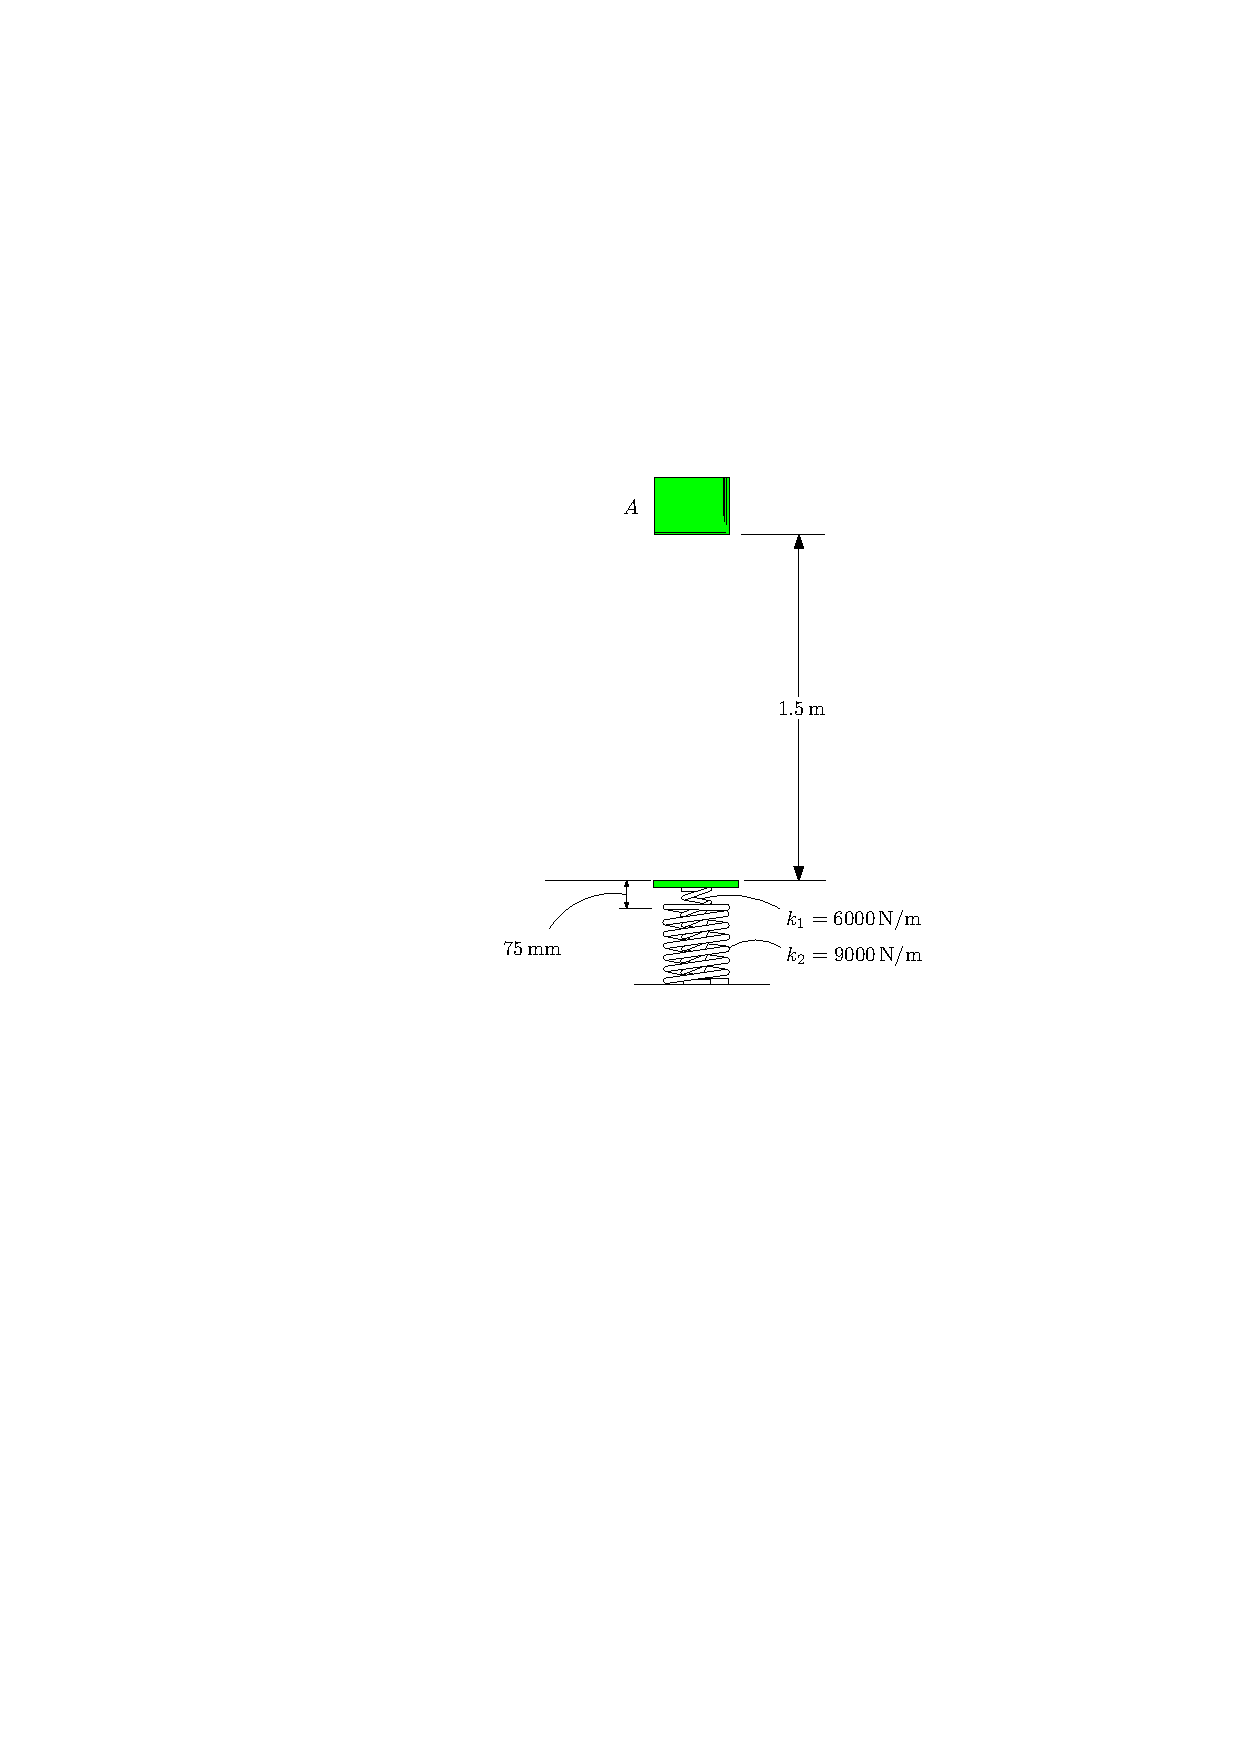
\includegraphics[scale=1.2]{images/draw_4.pdf}
\end{flushright}